\section{Realization}
%Focus generale sulle tecnologie utilizzate
In this section we outline the technical aspects concerning the realization of our framework. Therefore we first present the enabler technologies through which we instantiate the design principles presented in \cref{sec:design}. After that, we discuss the interaction workflow between the instantiated technologies. Finally, we show the implementation details.
\begin{figure}[t]
\centering
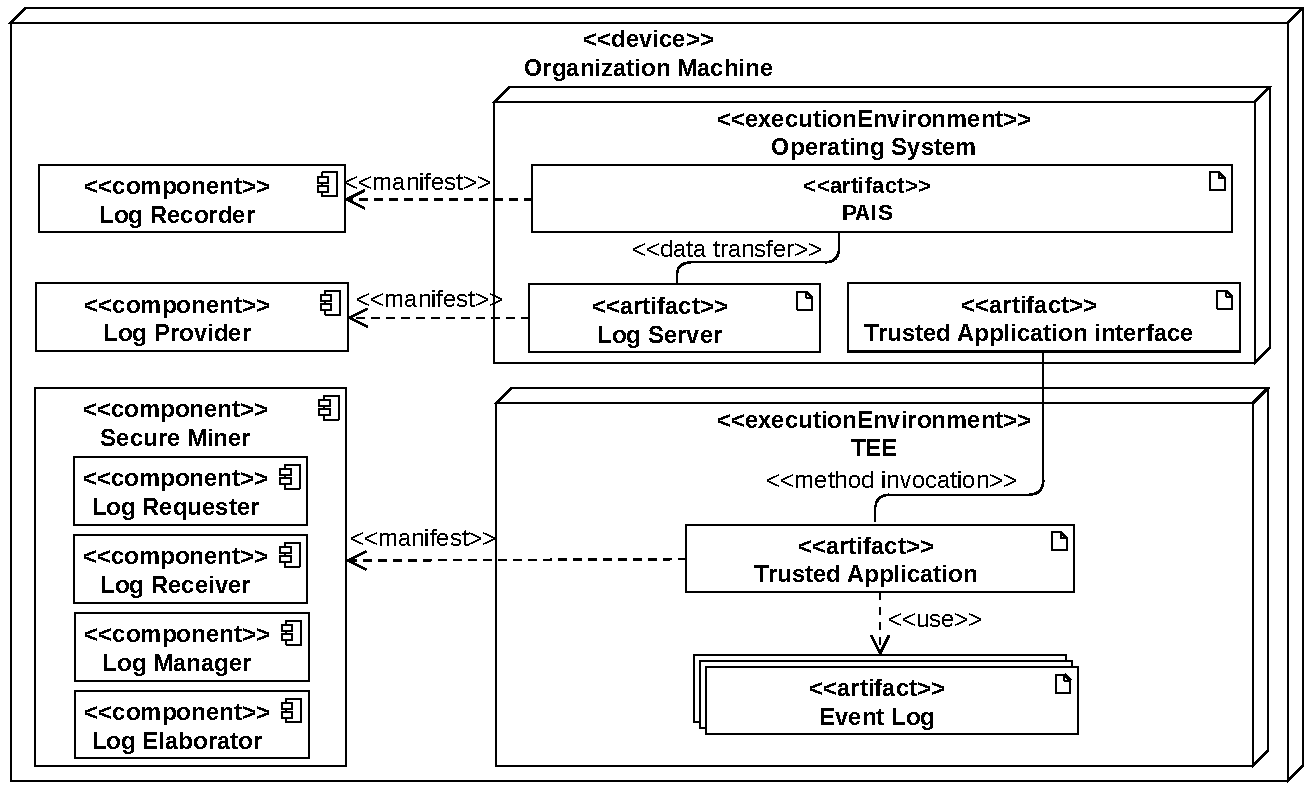
\includegraphics[width=10cm]{content/figures/deployment_diagram.pdf}
\caption{UML deployment diagram.}
\label{fig:deployment_diagram}
\end{figure}
\subsection{Deployment}
As follow, we bridge the gap between high-level system architecture and its practical realization. \cref{fig:deployment_diagram} depicts a \textit{UML deployment diagram} \cite{koch2002expressive} that aims to help with understanding the instantiated infrastrucuture. 

The \texttt{Organization Machine} represent the physical computation \textit{device} embracing the software and hardware entities of the company. The \texttt{Log Recorder}, the \texttt{Log Provider} and \texttt{Secure Miner} are included in the \texttt{Organization Machine} as abstract \textit{components} . These logical elements incorporate the core functionalities already discussed in \cref{sec:design}. The \texttt{Organization Machine} is characterized by two \textit{execution environment}s namely the \texttt{Operative System} and the \texttt{Trusted Execution Environment}.

Software entities that we expose to the users of the \texttt{Organization Machine} run inside the \texttt{Operative System}. We mainfest the functionalities offered by the \texttt{Log Recorder} in the \texttt{Process Aware Information System}  \cite{Dumas.etal/2018:FundamentalsofBPM}. These systems help users to handle business processes including accounting and resource management. In our solution, the \texttt{Process-Aware Information System} provides the \texttt{Log Server} access to event logs. \texttt{Log Servers} are web services which processes remote data request and provides event log to miners. We build this entities upon existing web standards such as HTTP, FTP and Goopher.

\texttt{Trusted Execution Environment}s are the core technologies of our solution. It creates a separated context from the normal \texttt{Operating System} to protect code and data through hardware-based security features in a reserved zone of the \texttt{Organization Machine}'s CPU. We leverage the security guarantees offered by this techonologies to instantiate a \texttt{Trusted Application} to fulfill the functionalities of the \texttt{Secure Miner} and its subcomponents. The \texttt{Trusted Application} collect the logic generate verifiable data request, receive event external logs, store them in the \texttt{Trusted Execution Environment}, and apply process mining algorithms. Procedures executed by the \texttt{Trusted Application} are tamperproof. The \texttt{Trusted Execution Environment} ensures that the code of the \texttt{Trusted Application} executed within it is protected from unauthorized accesses and malicious manipulations. We employ the isolated context of \texttt{Trusted Execution Environment} to store \texttt{Event Log}s of partner orgnizations inside the miner machine. The \texttt{Trusted Execution environment} provide mechanism to protect this sensitive information withoutg exposing it to the \texttt{Operative System}. The \texttt{Trusted Application} is the only entity that can access the \texttt{Event Log}s and feed them to process mining algorithms. Users can communicate with the \texttt{Trusted Application} via the \texttt{Trusted Application Interface}. The \texttt{Trusted Application} offer secure methods to safely receive information from  the \texttt{Operative System} and present the outputs of the computation. These methods are invoked by the \texttt{Trusted Application Interface} and instantiate the only communication channel to the \texttt{Trusted Application}.
%What the secure miner can do
%-TEEs ensure that the code and data executed within the environment are protected from unauthorized access
%TEEs provide mechanisms to protect sensitive data stored within the environment. Encryption and decryption operations can be performed securely without exposing the data to the less secure parts of the system.
%


%The \texttt{PAIS Interface} collects the logic to interact with the Process-aware Information Sytem (\texttt{PAIS}) of the \texttt{Organization}. \texttt{PAIS} systems help \texttt{Organization}s to handle business processes including accounting and resource management. The maintenance of event logs is the core tasks performed by these systems~\cite{Dumas.etal/2018:FundamentalsofBPM}. In our architecture, we generalize the interaction with \texttt{PAIS}s through the \texttt{PAIS Interface}. The \texttt{PAIS Interface} is queried by the local \texttt{Log Provider} for event logs to be fed into \texttt{Secure Miner}s.
\begin{figure}[t]
\centering
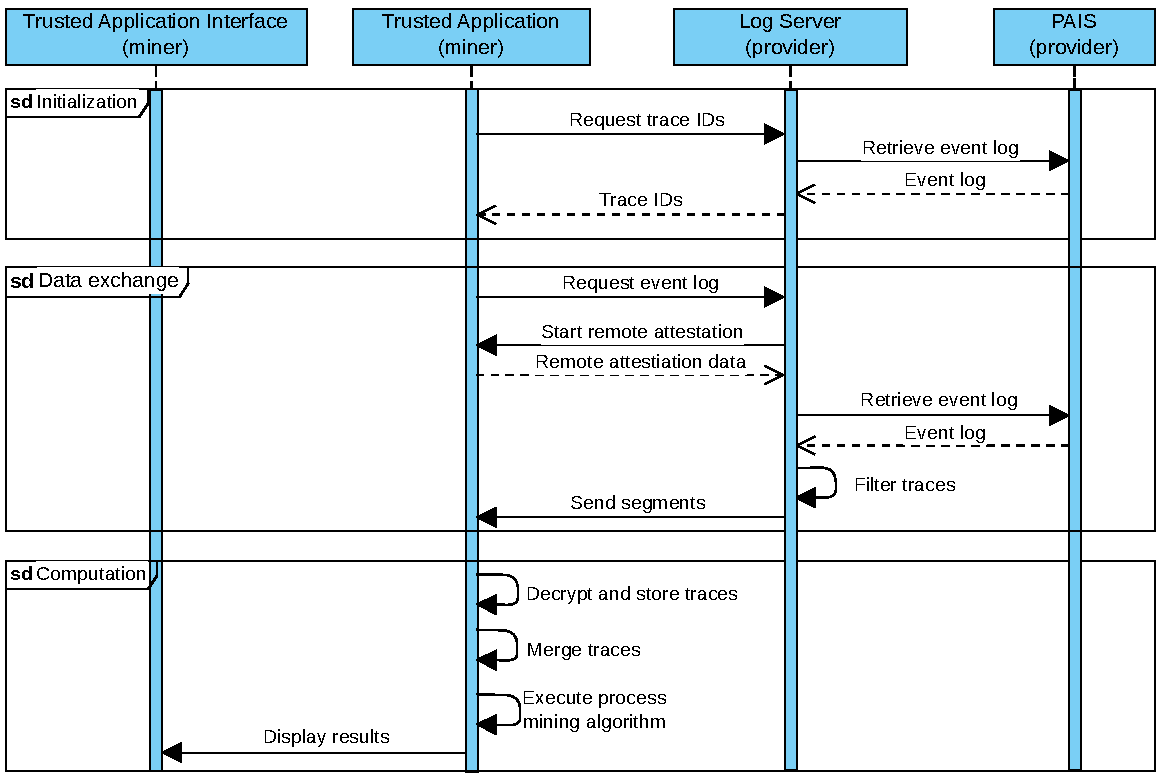
\includegraphics[width=10cm]{content/figures/sequence_diagram.pdf}
\caption{UML sequence diagram.}
\label{fig:sequence_diagram}
\end{figure}
\subsection{Workflow}
The parties involved in the process are a miner (i.e., an organization that execute process mining algorithms) and one or more providers (i.e., partner organizations that serve their event logs). We distinguish three different phases of the process namely the \textit{initialization}, the \textit{data exchange}, and the \textit{computation}.

\textbf{Initialization.} The procedure starts with the initialization phase, in which the miner's \texttt{Trusted Application} requests preliminary information from the providers' \texttt{Log Service} concerning the event logs of a shared business process. After the authentication of the sender, the involved \texttt{Log Service}s retrieve the local event log from the \texttt{Process-Aware Information System} and respond the miner by providing the list of trace ids recorded in the event log. Hence, the \texttt{Trusted Application} collect the responses and collect them in the \texttt{Trusted Execution Environment}

\textbf{Data exchange.} Once received the necessary information, the miner starts the data exchange procedure. Therfore, its \texttt{Trusted Application} sends log requests to \texttt{Log Servers}. Data requests include a list of trace ids and a segment size. Subsequently, \texttt{Log Server}s starts the \textit{remote attestation} procedure thanks to which the it can verify that the sender of the log request is actually a \texttt{Trusted Application} running inside a \texttt{Trusted Execution Environment} and belonging to a known organization. This operation involve the exchange of additional messages between the \texttt{Log Server} and the \texttt{Trusted Application}. If the procedure is successful, the identity of the miner is verified and its public key determined. After that, \texttt{Log Servers} retrieve the event log and filter its traces according to the trace ids sent by the \texttt{Trusted Application}. Filtered \texttt{Log Servers} are splitted in several segments whose dimension does not exceed the segment size sent by the miner in the initial request. Finally, \texttt{Log Servers} encrypts each segment and send them to the \texttt{Trusted Application}.

\textbf{Computation.}
\subsection{Implementation}
%\subsubsection{Event Log Generation}
%Tecnologie utilizzate
%Sintesi del processo di generazione dei log
%\subsubsection{Trusted Miner and Log Provider}
%Tecnologia TEE usata
%Linguaggio usato per programmare in TEE
%Algoritmo implementato
%Rappresentazioni intermedie (PNML, Petrinet, ecc...)
%Linguaggio Log provider
